\chapter{Properties of Logarithms}
%%%%%%%%%%%%%%% SECTION HEADER %%%%%%%%%%%%%%%%
\lhead{Properties of Logarithms}
\rhead{3}
%%%%%%%%%%%%%%%%%%% START %%%$%%%%%%%%%%%%%%%%%
\section{More properties}
We will discuss three important properties of logarithms. We can use them either to 
expand or condense logarithms. All of them can be proven using the exponent rules.
\begin{tcolorbox}[title= Rules of Logarithms, fonttitle=\bfseries, 
                  colframe=blue!70!black,colback=blue!5!white]
	\begin{align}
		\log_{b}(M\cdot N)&=\log_{b}M + \log_{b}N &	&\text{Product rule} \label{product}\\
		\log_{b}\left(\frac{M}{N}\right)&=\log_{b}M - \log_{b}N &	&\text{Quotient rule}\label{quotient}\\
		\log_{b}(M^{p})&=p\log_{b}M &	&\text{Power rule} \label{power}
	\end{align}
\end{tcolorbox}
% ========= NOTE
\begin{nt} The product rule is telling us that the logarithm of a product is the sum of 
logarithms. However, based on the quotient rule, the log of a quotient is the difference 
of logs. Regarding power rule, you can think of it as pulling the exponent in the front.
\end{nt}
% ==========
		\begin{figure}[H]
		 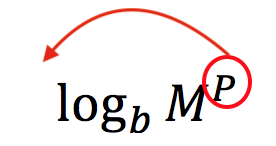
\includegraphics[width=3cm]{pics/power.png}
		 \centering
		 \caption{Power rule}
		\end{figure}
%
To \textbf{expand} a single logarithm follow these steps:
	\begin{itemize}
		\item First try to use either product rule \eqref{product} or quotient rule \eqref{quotient}	
		\item Then use power rule \eqref{power}
	\end{itemize}
%
    If you want to \textbf{condense} several logarithms as a single log, however, it is convenient to use the guidelines listed below for condensing logarithms:
    	\begin{itemize}
		\item First apply power rule to move out the number in front of the
			  logarithm to the exponent of variable
		\item Apply product or quotient rule to change the addition and subtraction
			  logarithms to the multiplication and division.
		\end{itemize}
% ============= EXAMPLE 1
\begin{exa}
	Expand each following logarithmic expression.
	\begin{multicols}{2}
	\begin{enumerate}[\bfseries a.]
	    \item $\log_{6}(7\cdot11)$
	    \item $\log_{}(100x)$
	    \item $\log_{8}\left(\frac{23}{x}\right)$
	    \item $\ln{\left(\frac{e^5}{11}\right)}$
	    \item $\log_{}(x+4)^2 $
	    \item $\log_{6}3^9 $
	    \item $\ln{\sqrt[3]{x}} $
	    \item $\log_{6}{36x} $
	\end{enumerate}
	\end{multicols}
\end{exa}
%
a.	\begin{align*}
		\log_{6}(7\cdot11)&         &       &\text{Use product rule \eqref{product}}\\
		\log_{6}7+\log_{6}11&       &       &\text{Our solution}\\
    \end{align*}
%
b.    \begin{align*}
		\log_{}(100x)&	            &       &\text{Use product rule \eqref{product}}\\
		\log_{}100+\log_{}x&	    &       &\text{We know $10^2=100$ so $\log_{}100=2$}\\
		2+\log_{}x&	                &      &\text{Our solution}\\
     \end{align*}
%
c.    \begin{align*}
		\log_{8}\left(\frac{23}{x}\right)&	&   &\text{Use quotient rule \eqref{quotient}}\\
		\log_{8}23-\log_{8}x&	            &   &\text{Our solution}\\
     \end{align*}
%
d.   \begin{align*}
		\ln{\left(\frac{e^5}{11}\right)}&	&   &\text{Use quotient rule \eqref{quotient}}\\
		\ln{e^5}-\ln{11}&          &   &\text{We are technically done!} \\
		                          &&   &\text{But we can find $\ln{e^5}$ by}\\
		                          &&   &\text{using the power rule \eqref{power}, first}\\
		5\ln{e}-\ln{11}&   &    &\text{then use identity \eqref{ID_1}}\\
		5(1)-\ln{11}&   &       &\text{Multiply}\\
		5-\ln{11}&      &       &\text{Our solution}\\	
     \end{align*}
%
e.    \begin{align*}
		\log_{}(x+4)&^2		&       &\text{Use power rule \eqref{power}}\\
		2\log_{}(x+4)&      &       &\text{Our Solution}\\
	  \end{align*}
%
f.	  \begin{align*}
		\log_{6}3^9&		&       &\text{Use power rule \eqref{power}}\\
		9\log_{6}(3)&		&       &\text{Our Solution}\\
	  \end{align*}
%
g.	  \begin{align*}
		\ln{\sqrt[3]{x}}&			&&\text{Rewrite in rational notation \eqref{rat_exp}}\\
		\ln{{x}^{\sfrac{1}{3}}}&	&&\text{Use power rule \eqref{power}}\\
		\frac{1}{3} \ln{x}&		    &&\text{Our Solution}\\
	 \end{align*}
%
h.  \begin{align*}
		\log_{6}{36x}&			    &&\text{Use product rule \eqref{product}}\\
		\log_{6}{36}+\log_{6}x&	    &&\text{6 to power 2 gives us 36, so $\log_{6}{36}=2$}\\
		2+\log_{6}x&                &&\text{Our solution}\\
	 \end{align*}
% ========== NOTE
\begin{nt}
As you observed in Example 1, in some cases you can simplify your answer more. You always 
need to keep asking yourself whether you can simplify it more.
\end{nt}
% ============= Example 2
\begin{exa}
	Write as each expression a single logarithm.
	\begin{enumerate}[\bfseries a.]
	    \item $\log_{}25+\log_{}4$
	    \item $2\ln{(x-3)}-\ln{x}$
	    \item $\frac{1}{4}\log_{b}x-2\log_{b}5-10\log_{b}y$
	\end{enumerate}
%
\end{exa}
The question is asking us to condense each expression.\\
 a.\begin{align*}
		\log_{}25+\log_{}4&	    &&\text{Use the product rule}\\
		\log_{}(25\cdot4)&		&&\text{Multiply}\\
		\log_{}(100)&			&&\text{Simplify, 100 is $10^2$}\\
		\log_{}(10^2)&			&&\text{Apply power rule}\\
		2\log_{}(10)&			&&\text{We know $\log_{}10=1$}
		\\
		2&						&&\text{Our Solution}\\
    \end{align*}
b.  \begin{align*}
		2\ln{(x-3)}-\ln{x}&		&&\text{Apply power rule}\\
		\ln{(x-3)^2}-\ln{x}&		&&\text{Use quotient rule}\\		
		\ln{\frac{(x-3)^2}{x}}&		&&\text{Our Solution}\\
    \end{align*}
c.  \begin{align*}
		\frac{1}{4}\log_{b}x-2\log_{b}5-10\log_{b}y&	&&\text{Apply power rule}\\
		%
		\log_{b}x^{1/4}-\log_{b}5^2-\log_{b}y^{10}&	&&\text{Use quotient rule on first two logs}\\
		%
		\log_{b}(\frac{x^{1/4}}{25})-\log_{b}y^{10}& &&\text{Apply quotient rule, again}\\
		%
		\log_{b}(\frac{x^{1/4}}{25y^{10}})& &&\text{Our Solution}\\	 
	\end{align*}
% ======== SECTION
\section{Change of base property}
We may often need to evaluate logarithms with other bases. In this case, we can change the base of a logarithm to any other base (including 10 and $e$), using the change-of-base property.For any logarithmic bases a and $N$, and any positive number $M$,
		\begin{equation}
			log_{N}M = \frac{\log_{b}M}{\log_{b}N}
		\end{equation}
In other words, the logarithm of M with base N is equal to the logarithm of M with any new base divided by the logarithm of N with that new base.
%
	\begin{figure}[H]
		 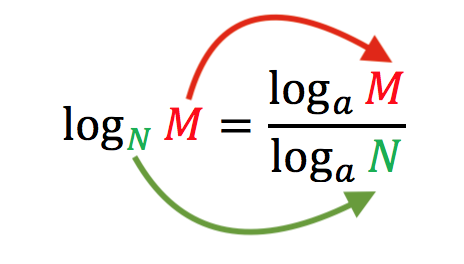
\includegraphics[width=5cm]{pics/change_base.png}
		 \centering
		 \caption{Arrows to help us remember: M goes up, N goes down.\\}
	\end{figure}
%


The change-of-base property is used to write a logarithm in terms of quantities that can 
be evaluated with a calculator. Because calculators contain keys for common (base 10) 
and natural (base $e$) logarithms, we will frequently introduce base 10 or base e. 
	\begin{table}[H]
	\caption{Change-of-base property: introducing common and natural log}
		\centering
		\begin{tabular}{ *{5}{c}}
		    \toprule
			Common logarithm		&&&&	Natural logarithm\\
			\hline \hline\\
			$\displaystyle log_{N}M = \frac{\log_{}M}{\log_{}N}$ & &&&
			$\displaystyle log_{N}M = \frac{\ln{M}}{\ln{N}}$\\[.4cm]
			\bottomrule
		\end{tabular}
	\end{table}
% ====== EXAMPLE
\begin{exa}
Use natural logarithms to evaluate $\log_{7}2506$. Round your answer to 2 decimal places.
\end{exa}
%
\begin{align*}
	\log_{7}2506 &		&&\text{Use change-of-base property}\\
	%
	\frac{\ln{2506}}{\ln{7}}&   &&\text{Use calculator to find each ln}\\[.2cm]
	%
	\frac{7.82644314}{1.94591015}&  &&\text{Divide} \\[.2cm]
	\approx 4.02&		&&\text{Our solution}
\end{align*}
% ======= EXAMPLE
\begin{exa}
Use common logarithms to evaluate $\log_{3}764$.
\end{exa}
%
\begin{align*}
	\log_{3}764 &		&&\text{Use change-of-base property}\\
	%
	\frac{\log_{}{764}}{\log_{}{3}}&   &&\text{Use calculator to find each log}\\[.2cm]
	%
	\frac{2.88309336}{0.47712125}&  &&\text{Divide} \\[0.2cm]
	\approx 6.04&		&&\text{Our solution}
\end{align*}